\chapter{Introduction}
\label{chap:intro}
\section{Motivation}

Since the dawn of human civilization, the capacity to traverse distances and transport resources has been the fundamental catalyst for societal evolution. From the establishment of ancient overland networks like the Silk Road to the mechanized leaps of the Industrial Revolution, the physical movement of people and products has dictated the rhythm of human progress. Transportation is not merely a mechanism of convenience; it is the circulatory system of the global economy, directly influencing the prosperity, resilience, and connectivity of nations. In the modern era, this system has grown into a staggering, deeply interconnected logistical network without which contemporary society would immediately stall.
\begin{figure}[H]
    \centering
    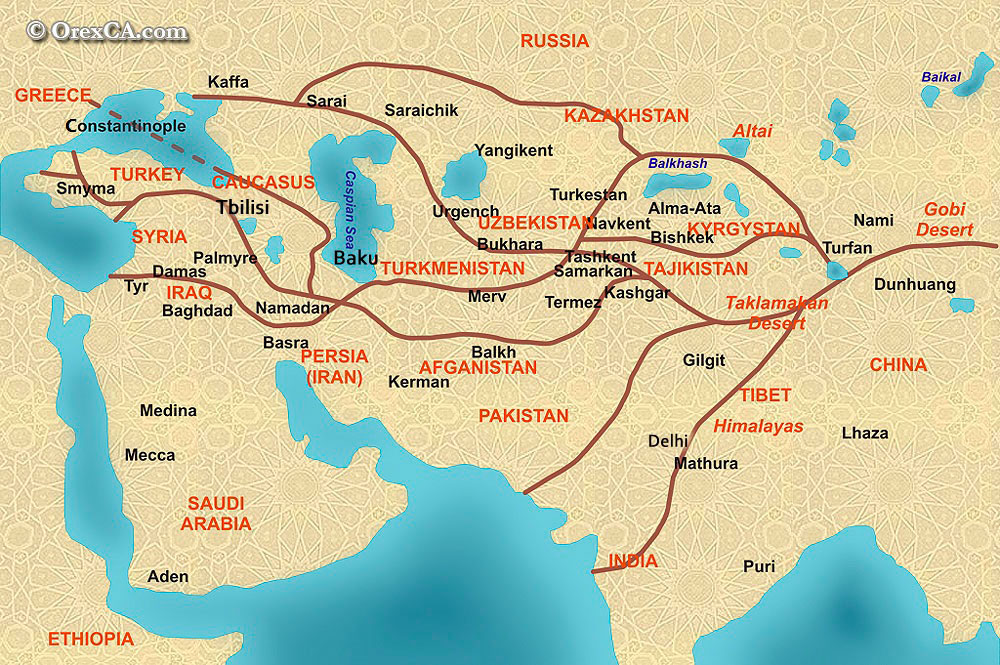
\includegraphics[width=0.5\linewidth]{Thesis Pictures/Silk Road Map.png}
    \caption{A map depicting the Silk Road}
    \label{fig:silk_road}
\end{figure}
Today, transportation vehicles remain an inescapable necessity of daily life, heavily dominated by land-based transit. The sheer volume of modern road transportation is immense. According to recent global logistics data, road freight facilitates the movement of more than 87 billion metric tons of goods annually, representing over 70\% of all inland freight moved globally\cite{itf_outlook_2023}. Furthermore, the relentless expansion of global trade and e-commerce has pushed fleet utilization to historical highs, underscoring the world's absolute reliance on commercial trucks and delivery vehicles to sustain supply chains.

On the passenger front, the dependence on land vehicles is equally overwhelming. According to the International Energy Agency (IEA), passenger cars dominate road transport demand, accounting for approximately 60\% to 65\% of all road energy use in advanced economies\cite{iea_transport_2025}. Whether facilitating daily workforce commutes, bridging rural divides, or enabling industrial logistics, road vehicles are the undisputed backbone of global mobility.

However, the astronomical scale of this mobility comes at a severe economic and environmental price. As global economic pressures and geopolitical uncertainties continue to rise, the cost of operating these vast fleets has become a critical vulnerability. The transportation sector currently accounts for nearly 30\% of total global energy demand. Alarmingly, road transport alone is responsible for roughly 45\% of global oil demand and over 25\% of the world's energy-related carbon dioxide emissions.

For freight operators, fuel often represents the single largest ongoing operating expense, meaning that volatile energy markets translate directly into inflated consumer prices and strained corporate profit margins. Similarly, for the everyday commuter, rising energy costs continually erode disposable income, making the baseline cost of moving from point A to point B an increasing financial burden.
\begin{figure}[H]
    \centering
    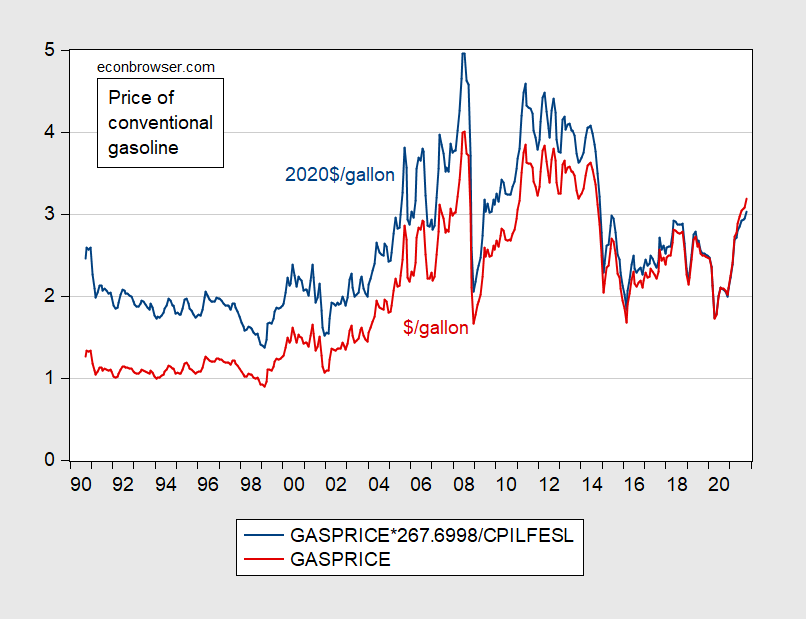
\includegraphics[width=0.5\linewidth]{Thesis Pictures/fuel prices.png}
    \caption{Fuel price trends since the 90s}
    \label{fig:placeholder}
\end{figure}
Consequently, this convergence of massive operational scale, heavy energy reliance, and volatile economic pressures has created a critical inflection point for modern engineering. It is no longer sufficient to merely expand transportation infrastructure; there is now a pressing, urgent need to fundamentally improve how efficiently energy is utilized and conserved within vehicle systems themselves. Driving mechanical and electrical efficiency—whether through powertrain optimization, aerodynamic refinements, or advanced energy recovery mechanisms—is no longer an environmental luxury. It is an economic imperative required to sustain the global mobility upon which human civilization relies.

Despite continuous advancements in automotive technology, the overall efficiency of conventional vehicles remains relatively low, typically ranging between 12 percent and 30 percent\cite{doe_ev_efficiency}. This indicates that a large portion of the energy supplied to the vehicle is not effectively used for propulsion. Instead, it is lost in forms such as heat, friction, and mechanical vibrations. These losses highlight a major opportunity for improvement, since recovering even a small portion of this wasted energy can lead to noticeable gains in overall efficiency.
\begin{figure}[H]
    \centering
    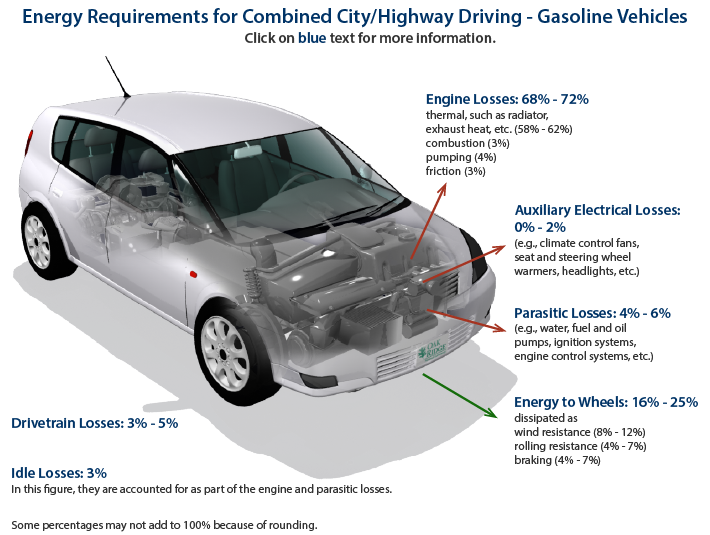
\includegraphics[width=0.75\linewidth]{Thesis Pictures/vehicle efficiency.png}
    \caption{Energy losses in cars}
    \label{fig:energy_cars}
\end{figure}
Moreover, the suspension system plays a dual role in vehicle operation that extends beyond mechanical support. In terms of safety, the suspension governs the dynamic contact force between the tyre and road surface. Adequate tyre contact is essential for maintaining steering response, braking effectiveness, and lateral stability, particularly during emergency maneuvers or adverse road conditions. A reduction in tyre dynamic load, or worse, intermittent loss of road contact, directly compromises the driver's ability to control the vehicle and increases the risk of accidents. In terms of occupant comfort and health, prolonged exposure to whole-body vibration transmitted through the suspension has been linked to fatigue, reduced driver alertness, and musculoskeletal stress, as quantified by ISO 2631-1 which establishes human tolerance limits for vertical acceleration exposure. These considerations establish that the suspension system is not merely a passive structural component but an active determinant of both vehicle safety and occupant wellbeing. Consequently, any strategy that modifies suspension behaviour in pursuit of energy recovery must demonstrate that it does not degrade road-holding performance or increase vibration exposure beyond acceptable limits. This requirement motivates the need for an intelligent control framework capable of simultaneously optimising energy regeneration and suspension performance rather than treating them as independent objectives.

In response to these challenges, researchers and engineers have increasingly focused on the development of regenerative techniques. These techniques are designed to capture energy that would otherwise be lost and convert it into a useful form. One of the most widely known applications is regenerative braking, where the kinetic energy of a moving vehicle during deceleration is converted into electrical energy and stored for later use. More generally, regenerative systems can be applied to any part of a vehicle where energy is dissipated without serving a useful purpose.
\begin{figure}[H]
    \centering
    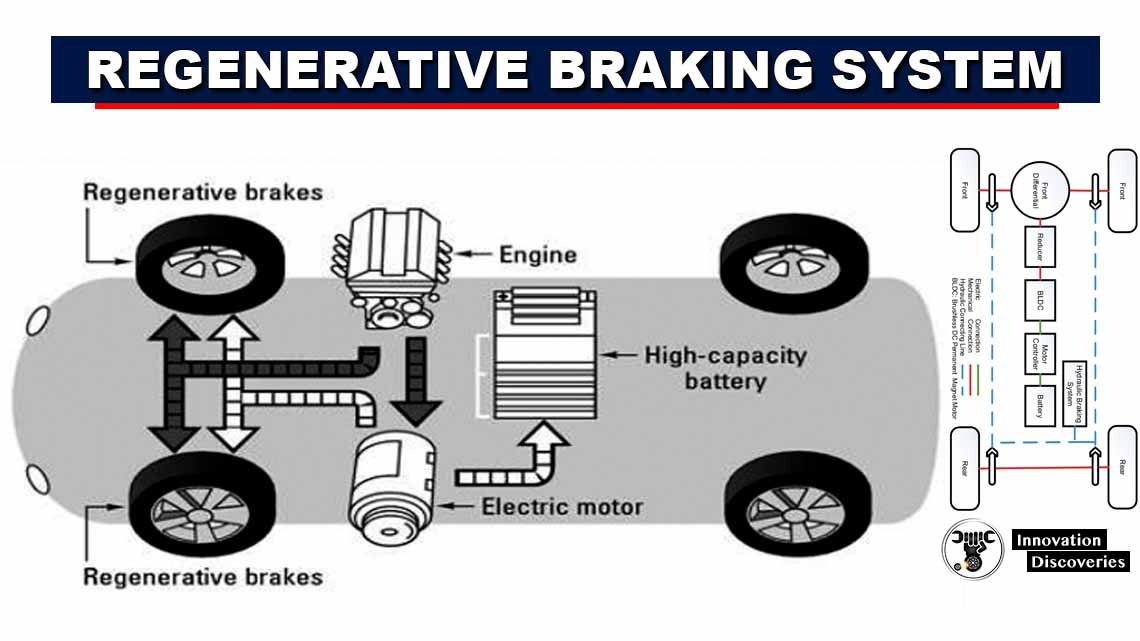
\includegraphics[width=0.5\linewidth]{Thesis Pictures/Regenerative Braking System Explained.jpg}
    \caption{Topology of a regenerative braking system}
    \label{fig:regen_braking}
\end{figure}
With the rapid growth of electric vehicles, the importance of regenerative technologies has increased even further. Unlike conventional vehicles, electric vehicles rely entirely on electrical energy stored in batteries, which makes efficient energy management essential. In this context, regenerative techniques are primarily used to convert wasted mechanical energy into electrical energy that can be stored and reused. This process helps extend the driving range of the vehicle, reduces overall energy consumption, and supports more sustainable operation.

Building on this concept, recent research has explored the possibility of applying regenerative principles beyond braking systems to other components of the vehicle. One particularly promising area is the suspension system, which continuously dissipates energy while maintaining ride comfort and vehicle stability. By integrating electromechanical mechanisms along with suitable control strategies, it becomes possible not only to improve suspension performance but also to recover energy that would otherwise be lost.


\section{Project Aim and Novelty}
\label{sec:aim}
% ------------------------------------------------------------

Contemporary vehicle suspension systems face a fundamental conflict
between three competing engineering objectives: ride comfort, which
demands soft, compliant damping to isolate the vehicle body from road
irregularities; road holding, which demands stiff, responsive damping
to maintain tyre contact with the road surface; and energy efficiency,
which demands that the mechanical vibration energy dissipated by the
damper be harvested and returned to the vehicle's electrical system
rather than lost as heat. Conventional passive dampers cannot
simultaneously satisfy all three objectives, and active systems that
do so consume more electrical energy than they recover. Semi-active
energy-regenerative suspension, in which a linear electromagnetic motor
replaces the oil damper and operates simultaneously as a controllable
force actuator and an electrical generator, offers a principled
resolution to this conflict — provided that an appropriate control
architecture is designed to coordinate the mechanical and electrical
subsystems.
\begin{figure}[H]
    \centering
    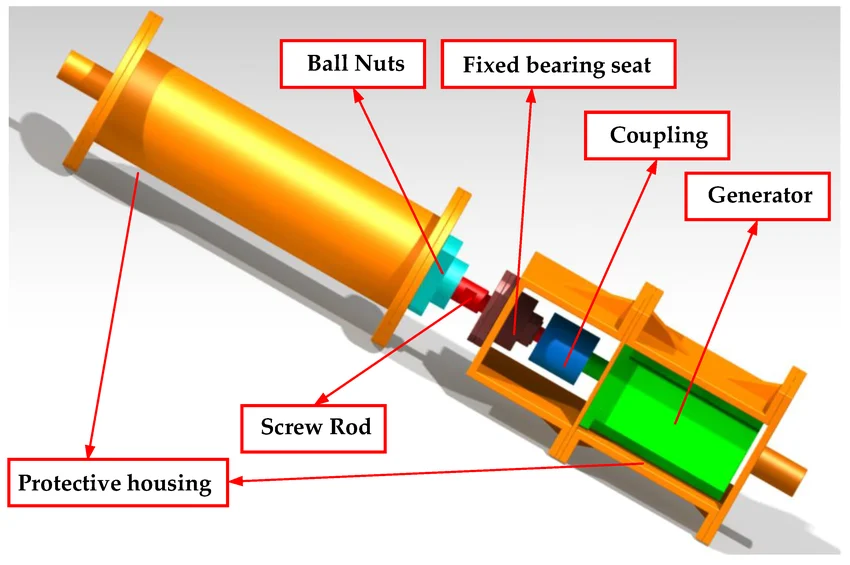
\includegraphics[width=0.5\linewidth]{Thesis Pictures/Em Damper Structure (1).png}
    \caption{Structure of an electromagnetic damper}
    \label{fig:em_damper}
\end{figure}
The electromagnetic damper introduces a nonlinear, variable-structure
power conversion stage between the motor terminals and the energy
storage element. Specifically, the unidirectional boost--buck converter
that interfaces the motor to the battery must operate in one of three
distinct modes — boost, buck, or passive — depending on the
instantaneous motor velocity and the required damping force. The
transition between these modes is governed by nonlinear switching
boundaries that depend on circuit parameters, battery voltage, and the
motor back-electromotive force. Conventional linear controllers such
as proportional--integral regulators cannot guarantee stable current
tracking across all three operating regions, since the converter
dynamics change structure at each mode boundary.

Tha aim of this thesis is to propose a model predictive controller as the outer-loop
force reference generator, incorporating speed-adaptive performance
weights to replace the fixed hybrid skyhook-groundhook law of \cite{shi2019research}.
The identified gap in the existing literature is the absence of a
unified control framework that explicitly coordinates ride comfort and
road-holding performance across the full suspension operating frequency
range, and adapts its control priority continuously to the dominant
excitation frequency without requiring structural modification or
driver intervention. Existing approaches based on fixed
hybrid skyhook-groundhook laws produce static, memoryless force references that 
do not adapt to the frequency content of the road excitation, frequently command 
unachievable active forces that must be abruptly clipped by the plant, and 
apply identical damping trade-offs regardless of whether the system is 
operating near the sprung mass resonance at \SI{1.3}{\hertz} or the unsprung mass
resonance at \SI{10.9}{\hertz}.

The proposed MPC formulation addresses these limitations. By solving a
constrained finite-horizon quadratic programme at each sampling instant,
the MPC computes a reference force that minimises a weighted combination
of body acceleration and tyre dynamic load, subject to explicit
constraints on force direction, dead-zone exclusion, and force rate-of-change. 
The performance weights are scheduled continuously as sigmoid functions of the 
vehicle's longitudinal speed, automatically emphasising comfort attenuation near the
sprung mass resonance and road-holding performance near the unsprung
mass resonance. Harvested power is evaluated as an independent
performance metric alongside body acceleration and tyre dynamic load,
enabling a transparent three-way assessment of the control trade-off
without conflating the optimisation objective with the evaluation
criterion.

The specific objectives of this thesis are:

\begin{enumerate}
    \item To derive and validate a first-principles mathematical model
          of the quarter-car suspension, linear electromagnetic motor,
          bridge rectifier, and unidirectional boost--buck converter
          operating under the continuous conduction mode averaged
          model assumption.
    \item To implement the sliding mode current controller of
          \cite{shi2019research} that achieves robust inductor current tracking
          across the boost, buck, and passive operating regions of the
          converter, providing the inner-loop foundation for the
          proposed outer-loop MPC strategy.
    \item To design and implement a speed-adaptive model predictive
          force reference generator with sigmoid-scheduled performance
          weights, and to demonstrate that it produces lower body
          acceleration near sprung mass resonance and lower tyre dynamic
          load near unsprung mass resonance compared to the fixed
          hybrid skyhook-groundhook baseline of \cite{shi2019research}.
        \item To evaluate the proposed controller's reference against the hybrid skyhook-groundhook's reference across six standardised test scenarios — sinusoidal
          excitation at \SI{1.3}{\hertz} and \SI{10.9}{\hertz}, and
          ISO 8608 Class~B and Class~D random road profiles at low and
          high vehicle speeds — using body acceleration and tyre dynamic
          load as the primary performance metrics.
    \item To evaluate the proposed controller's ability to actualize the force due to converter dynamics against the hybrid skyhook-groundhook's actualization
           across six standardised test scenarios — sinusoidal
          excitation at \SI{1.3}{\hertz} and \SI{10.9}{\hertz}, and
          ISO 8608 Class~B and Class~D random road profiles at low and
          high vehicle speeds — using body acceleration, tyre dynamic
          load, and harvested power as the primary performance metrics.
    \item To evaluate the proposed controller against passive damping, and the hybrid skyhook-groundhook
          baseline across six standardised test scenarios — sinusoidal
          excitation at \SI{1.3}{\hertz} and \SI{10.9}{\hertz}, and
          ISO 8608 Class~B and Class~D random road profiles at low and
          high vehicle speeds — using body acceleration, tyre dynamic
          load, and harvested power as the primary performance metrics.
\end{enumerate}